\documentclass[12pt]{article}
\usepackage[pdftex]{graphicx}
\newcommand{\kg}{\mathrm{kg}}
\newcommand{\m}{\mathrm{m}}
\newcommand{\cm}{\mathrm{cm}}
\newcommand{\mm}{\mathrm{mm}}
\newcommand{\km}{\mathrm{km}}
\newcommand{\mi}{\mathrm{mi}}
\newcommand{\s}{\mathrm{s}}
\newcommand{\ms}{\mathrm{ms}}
\newcommand{\h}{\mathrm{h}}
\newcommand{\N}{\mathrm{N}}
\newcommand{\J}{\mathrm{J}}
\newcommand{\W}{\mathrm{W}}
\newcommand{\hp}{\mathrm{hp}}
\newcommand{\rad}{\mathrm{rad}}
\newcounter{problem}
\stepcounter{problem}
\newcounter{answer}[problem]
\newenvironment{problem}{\noindent\begin{minipage}{\textwidth}\sloppy\sloppypar\raggedright\textbf{\theproblem.}\refstepcounter{problem}\stepcounter{answer}---}{\end{minipage}\vspace{2ex}}
\newcommand{\source}[1]{[{#1}]}
\newenvironment{answers}{\\}{}
\newcommand{\answer}[1]{\textbf{\Alph{answer}:}\refstepcounter{answer}~\mbox{#1\hspace{3ex}}}
\begin{document}

\section*{NYU General Physics 1---Final Exam}

\begin{problem}
  \source{from lecture 2011-09-06} What is the mass of a cubic
  kilometer (a cube one km on a side) of water?
  \begin{answers}
    \answer{$10^{6}\,\kg$}
    \answer{$10^{8}\,\kg$}
    \answer{$10^{10}\,\kg$}
    \answer{$10^{12}\,\kg$}
    \answer{nowhere near any of these}
  \end{answers}
\end{problem}

\begin{problem}
  \source{from lecture 2011-09-08} A dense, heavy ball marked ``1''
  takes time $t_1$ to fall from a height of $1\,\m$, and an identical
  ball marked ``2'' takes time $t_2$ to fall from a height of $4\,\m$,
  both near the surface of the Earth.  If air resistance is not a
  factor, what is $t_1 / t_2$?
  \begin{answers}
    \answer{1}
    \answer{0.5}
    \answer{0.25}
    \answer{0.125}
    \answer{none of these}
  \end{answers}
\end{problem}

\begin{problem}
  \source{from lecture 2011-09-13} A girl throws a stone at an angle
  $\theta$ to the horizontal, so it flies upwards and to the right.
  Subsequently, because of gravity, it travels on a parabolic
  trajectory.  Precisely at the top of its parabolic trajectory, when
  it is exactly at its highest point, what is the acceleration of the
  stone?  Ignore air resistance.
  \begin{answers}
    \answer{0}
    \answer{$9.8\,\m\,\s^{-2}$ to the right}
    \answer{$9.8\,\m\,\s^{-2}$ to the left}
    \answer{$9.8\,\m\,\s^{-2}$ straight down}
    \answer{not enough information to say}
  \end{answers}
\end{problem}

\begin{problem}
  \source{from lecture 2011-09-15} A car, starting at rest,
  accelerates at a constant acceleration of $0.5\,\m\,\s^{-2}$ in the
  $x$ direction for $10\,s$.  How far does the car go during this
  $10\,\s$ period?
  \begin{answers}
    \answer{$0.5\,\m$}
    \answer{$5\,\m$}
    \answer{$10\,\m$}
    \answer{$25\,\m$}
    \answer{$50\,\m$}
  \end{answers}
\end{problem}

\begin{problem}
  \source{from lecture 2011-09-20} A block is placed on a frictionless
  inclined plane and released.  After release, if we ignore air
  resistance, how many forces are there to consider?  That is, how
  many non-zero forces are there on the free-body diagram for the block?
  \begin{answers}
    \answer{1}
    \answer{2}
    \answer{3}
    \answer{4}
    \answer{more than 4}
  \end{answers}
\end{problem}

\begin{problem}
  \source{from lecture 2011-09-27} An airplane turns in a horizontal
  turn---turns without gaining or losing altitude---by banking.  You
  can think of the airplane as having four forces acting on it:
  Gravity $m\,\vec{g}$, a combined normal force $\vec{N}$ coming from
  the two wings, a thrust force driving the plane through the air, and
  a drag force.  What is true as it is turning in its banked turn?
  \begin{answers}
    \answer{$|\vec{N}|>|m\,\vec{g}|$}
    \answer{$|\vec{N}|<|m\,\vec{g}|$}
    \answer{$\vec{N}+m\,\vec{g}=0$}
    \answer{The net force is in the vertical direction.}
    \answer{None of the above are true.}
  \end{answers}
\end{problem}

\begin{problem}
  \source{from lecture 2011-09-29} A textbook of mass $m$ is dropped
  from a high height onto a hard surface.  When it hits the surface,
  it is initially moving quickly (downwards) but it rapidly changes
  its velocity (it bounces!).  While it is in contact with the
  surface---while it is bouncing---or changing its velocity---it is
  subject to a contact force $\vec{N}$ that obeys the following:
  \begin{answers}
    \answer{$\vec{N}$ acts downwards and $|\vec{N}| > |m\,\vec{g}|$}
    \answer{$\vec{N}$ acts downwards and $|\vec{N}| = |m\,\vec{g}|$}
    \answer{$\vec{N}$ acts upwards and $|\vec{N}| = |m\,\vec{g}|$}
    \answer{$\vec{N}$ acts upwards and $|\vec{N}| > |m\,\vec{g}|$}
    \answer{none of these is true}
  \end{answers}
\end{problem}

\begin{problem}
  \source{from lecture 2011-10-06} In lecture, Prof Hogg swung a full
  coffee cup over his head on a circular arc.  Why did the coffee stay
  in the cup when it was directly above his head?
  \begin{answers}
    \answer{The cup was accelerating downwards with $|\vec{a}|>|\vec{g}|$.}
    \answer{The cup was accelerating downwards with $|\vec{a}|<|\vec{g}|$.}
    \answer{The cup was applying an upward force on the coffee.}
    \answer{The cup was applying no force on the coffee.}
    \answer{none of these}
  \end{answers}
\end{problem}

\begin{problem}
  \source{from lecture 2011-10-13} We considered a block sliding down
  a frictionless hill and off a frictionless jump.  The block flew up
  into the air, but it did not return to the height from which it
  started.  Why not?
  \begin{answers}
    \answer{Energy was not conserved.}
    \answer{The block lost energy to heat during its slide.}
    \answer{Not all of the potential energy was converted into kinetic energy.}
    \answer{After the jump, the horizontal component of velocity is constant.}
    \answer{There are energies other than kinetic and potential to consider.}
  \end{answers}
\end{problem}

\begin{problem}
  \source{from lecture 2011-10-18} A bullet lodged in a block.  What
  statement about the collision is true?
  \begin{answers}
    \answer{It was elastic because energy was conserved.}
    \answer{It was inelastic because energy was not conserved.}
    \answer{It was elastic because kinetic energy was conserved.}
    \answer{It was inelastic because kinetic energy was not conserved.}
    \answer{none of these}
  \end{answers}
\end{problem}

\begin{problem}
  \source{from lecture 2011-10-20} A block of mass $m_1=1\,\kg$
  moves at speed $|\vec{v}_1|=3\,\m\,\s^{-1}$ in the positive-$x$
  direction; another block of mass $m_2=0.5\,\kg$ moves at speed
  $|\vec{v}_2|=4\,\m\,\s^{-1}$ in the negative-$x$ direction.  What is
  the center-of-mass velocity of the two-block system?
  \begin{answers}
    \answer{$0.667\,\m\,\s^{-1}$ in the positive-$x$ direction}
    \answer{$1.0\,\m\,\s^{-1}$ in the positive-$x$ direction}
    \answer{$3.333\,\m\,\s^{-1}$ in the positive-$x$ direction}
    \answer{$5.0\,\m\,\s^{-1}$ in the positive-$x$ direction}
    \answer{nowhere near any of these}
  \end{answers}
\end{problem}

\begin{problem}
  \source{from lecture 2011-10-25} In lecture we thought about having
  a heavy mass $M$ on a light table-top supported by two sawhorses
  separated by a distance $L=100\,\cm$.  If you want the leftmost
  sawhorse to take roughly 2/3 of the weight, where should you put the
  mass?
  \begin{answers}
    \answer{more-or-less right over the left support}
    \answer{about $25\,\cm$ to the right of the left support}
    \answer{about $33\,\cm$ to the right of the left support}
    \answer{about $50\,\cm$ to the right of the left support}
    \answer{more than $50\,\cm$ to the right of the left support}
  \end{answers}
\end{problem}

\begin{problem}
  \source{from lecture 2011-11-01} Dimensionally, the fundamental
  frequency of a guitar string of length $L$ with mass $M$ at tension
  $T$ must be
  \begin{answers}
    \answer{$\displaystyle f = \frac{1}{2}\,\sqrt{\frac{M}{T\,L}}$}
    \answer{$\displaystyle f = \frac{1}{2}\,\sqrt{\frac{L}{M\,T}}$}
    \answer{$\displaystyle f = \frac{1}{2}\,\sqrt{\frac{T}{M\,L}}$}
    \answer{$\displaystyle f = \frac{1}{2}\,\sqrt{\frac{T\,L}{M}}$}
    \answer{none of these}
  \end{answers}
\end{problem}

\begin{problem}
  \source{from lecture 2011-11-10} You have a harmonic oscillator
  oscillating according to the following formula for position as a function of time:
  $$x = A\,\cos(\omega\,t + \phi)$$ What is the kinetic energy as a
  function of time?
  \begin{answers}
    \answer{$\displaystyle K = \frac{1}{2}\,m\,A^2\,\sin^2(\omega\,t + \phi)$}
    \answer{$\displaystyle K = \frac{1}{2}\,m\,A^2\,\cos^2(\omega\,t + \phi)$}
    \answer{$\displaystyle K = \frac{1}{2}\,m\,\omega^2\,A^2\,\sin^2(\omega\,t + \phi)$}
    \answer{$\displaystyle K = \frac{1}{2}\,m\,\omega^2\,A^2\,\cos^2(\omega\,t + \phi)$}
    \answer{none of these}
  \end{answers}
\end{problem}

\begin{problem}
  \source{from lecture 2011-11-15} How far does a traveling sinusoidal
  wave pattern of frequency $f$ traveling at speed $v$ travel in one
  period $T$?
  \begin{answers}
    \answer{$v\,f$}
    \answer{$\displaystyle\frac{f}{v}$}
    \answer{$\displaystyle\frac{1}{f}$}
    \answer{one wavelength}
    \answer{none of these}
  \end{answers}
\end{problem}

\begin{problem}
  \source{from lecture 2011-11-17} In lecture we made a standing wave
  by adding together two traveling waves.  These waves had the
  following properties.  \emph{Hint: Recall that at certain particular
    times, the two waves summed to exactly zero.}
  \begin{answers}
    \answer{same period, same amplitude, different directions of travel}
    \answer{same period, different amplitude, different directions of travel}
    \answer{different period, same amplitude, different directions of travel}
    \answer{different period, different amplitude, same direction of travel}
    \answer{none of these}
  \end{answers}
\end{problem}

\begin{problem}
  \source{from lecture 2011-11-22} A one-atmosphere pressure
  difference can be provided by $10\,\m$ of water or $0.76\,\m$ of
  mercury.  What is the origin of this difference between water and
  mercury?
  \begin{answers}
    \answer{$P\,V=n\,R\,T$ means smaller volume makes for higher pressure}
    \answer{the gravitational acceleration $\vec{g}$ is bigger for mercury}
    \answer{mercury is more than ten times more dense than water}
    \answer{the water is below sea level, but the mercury is above it}
    \answer{none of these}
  \end{answers}
\end{problem}

\begin{problem}
  \source{from lecture 2011-11-29} A helium balloon is floating in the
  middle of a stationary, sealed (airtight), air-filled bus parked on
  Broadway.  The driver starts the bus and accelerates forwards for
  many seconds.  During this long period of steady acceleration, how
  does the balloon move, relative to the bus?
  \begin{answers}
    \answer{the balloon moves towards the front of the bus}
    \answer{the balloon stays where it is}
    \answer{the balloon moves towards the back of the bus}
    \answer{more information is needed to answer this question}
  \end{answers}
\end{problem}

\begin{problem}
  \source{from lecture 2011-12-01} A cylindrical pipe has constant
  cross-sectional area (constant radius $R$).  Incompressible fluid is
  forced into one end at a particular rate $\Gamma$ (volume per time).
  What is the flow velocity in the pipe?
  \begin{answers}
    \answer{$\displaystyle v = 2\pi\,R\,\Gamma$}
    \answer{$\displaystyle v = \pi\,R^2\,\Gamma$}
    \answer{$\displaystyle v = \frac{\Gamma}{2\pi\,R}$}
    \answer{$\displaystyle v = \frac{\Gamma}{\pi\,R^2}$}
    \answer{none of these}
  \end{answers}
\end{problem}

\begin{problem}
  \source{from lecture 2011-12-06} If there is a horizontal pressure
  gradient in a fluid (that is, if the pressure is higher at one point
  $P$ than it is at some other point $Q$ at the same altitude or
  height), then which of the following must be true?  Assume that the
  acceleration due to gravity $\vec{g}$ points directly downwards
  (that is, vertically).
  \begin{answers}
    \answer{the fluid must be compressible}
    \answer{there must be a horizontal acceleration}
    \answer{the fluid must be flowing in a pipe}
    \answer{none of these}
    \answer{actually, this situation cannot happen}
  \end{answers}
\end{problem}

\begin{problem}
  \source{from lecture 2011-12-13} A surface tension $\sigma$ is a
  force per unit length.  If $L$ has dimensions of length, which of
  these is an energy?
  \begin{answers}
    \answer{$\sigma$}
    \answer{$\sigma\,L$}
    \answer{$\sigma\,L^2$}
    \answer{$\sigma\,L^3$}
    \answer{none of these}
  \end{answers}
\end{problem}

\begin{problem}
  \source{from problem set 1, problem 1} What, approximately, is the
  density of money?
  \begin{answers}
    \answer{$0.1\,\kg\,\m^{-3}$}
    \answer{$10\,\kg\,\m^{-3}$}
    \answer{$1000\,\kg\,\m^{-3}$}
    \answer{$10^5\,\kg\,\m^{-3}$}
    \answer{none of these}
  \end{answers}
\end{problem}

\begin{problem}
  \source{from problem set 2, problem 1} A dragster travels 0.25\,mi
  in 5.5\,s, starting from rest.  Under the assumption of constant
  acceleration, what is the time it takes the dragster to go half-way;
  that is, how many seconds does it take to go the first 0.125\,mi?
  \begin{answers}
    \answer{substantially less than $1.38\,\s$}
    \answer{$1.38\,\s$}
    \answer{$2.75\,\s$}
    \answer{$3.9\,\s$}
    \answer{substantially more than $3.9\,\s$}
  \end{answers}
\end{problem}

\begin{problem}
  \source{from problem set 2, problem 2} A rock is thrown directly
  upwards at $3\,\m\,\s^{-1}$.  What velocity will it have after
  $1\,\s$?  Calculate for the gravitational trajectory but ignore air
  resistance.
  \begin{answers}
    \answer{$13\,\m\,\s^{-1}$ upwards}
    \answer{$3\,\m\,\s^{-1}$ upwards}
    \answer{$3\,\m\,\s^{-1}$ downwards}
    \answer{$7\,\m\,\s^{-1}$ downwards}
    \answer{nothing near any of these}
  \end{answers}
\end{problem}

%% \begin{problem}
%%   \source{from problem set 3, problem 1} The Space Station orbits
%%   about $300\,\km$ above the surface of the Earth.  What is the radius
%%   of its orbit, roughly?
%%   \begin{answers}
%%     \answer{$300\,\km$}
%%     \answer{$1300\,\km$}
%%     \answer{$6700\,\km$}
%%     \answer{$600,300\,\km$}
%%     \answer{nowhere near any of these}
%%   \end{answers}
%% \end{problem}

\begin{problem}
  \source{from problem set 3, problem 2} What is the tension T in this
  problem?\\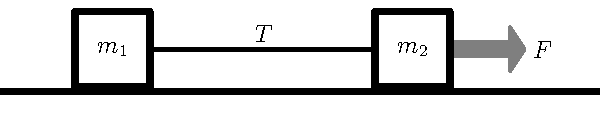
\includegraphics{../py/stringblocks.pdf}
  \begin{answers}
    \answer{$\displaystyle m_1\,g$}
    \answer{$\displaystyle m_2\,g$}
    \answer{$\displaystyle F$}
    \answer{$\displaystyle F\,\frac{m_1}{m_1+m_2}$}
    \answer{$\displaystyle F\,\frac{m_2}{m_1+m_2}$}
  \end{answers}
\end{problem}

\begin{problem}
  \source{from problem set 4, problem 1} A block of mass $m$ sits on a
  plane inclined at an angle of $\theta=20\,\deg$ to the horizontal.
  There is a coefficient of friction $\mu=0.9$ between the block and
  the plane.  What is the magnitude of the frictional force?
  \begin{answers}
    \answer{$m\,g\,\cos\theta$}
    \answer{$m\,g\,\sin\theta$}
    \answer{$\mu\,m\,g\,\cos\theta$}
    \answer{$\mu\,m\,g\,\sin\theta$}
    \answer{$\mu\,m\,g\,\tan\theta$}
  \end{answers}
\end{problem}

\begin{problem}
  \source{from problem set 5, problem 1} The driver of a car traveling
  east slams on the brakes, so that the car goes through a period of
  rapid deceleration.  The total force on the ground from the car must
  \begin{answers}
    \answer{have a downwards component and an eastwards component}
    \answer{have a downwards component and a westward component}
    \answer{have an upwards component and an eastwards component}
    \answer{have an upwards component and a westward component}
  \end{answers}
\end{problem}

\begin{problem}
  \source{from problem set 5, problem 3} Which of these does
  \emph{not} have units of energy?  In these formulae, $m$ is a mass,
  $v$ is a speed, $P$ is a pressure, $L$ is a length, and $F$ is a
  force.
  \begin{answers}
    \answer{$m\,v$}
    \answer{$m\,v^2$}
    \answer{$P\,L^3$}
    \answer{$F\,L$}
    \answer{none of these}
  \end{answers}
\end{problem}

\begin{problem}
  \source{from problem set 6, problem 1} If a $50\,\kg$ student climbs
  9 flights of stairs, about how much work does she do?
  \begin{answers}
    \answer{$50\,\J$}
    \answer{$500\,\J$}
    \answer{$1500\,\J$}
    \answer{$15,000\,\J$}
    \answer{none of these}
  \end{answers}
\end{problem}

\begin{problem}
  \source{from problem set 7, problem 1} Which of these figures---cut
  from a sheet of constant-thickness aluminum---has its center of
  mass at the point $(x,y) = (-1/3,-1/3)\,\cm$?
  \begin{answers}
  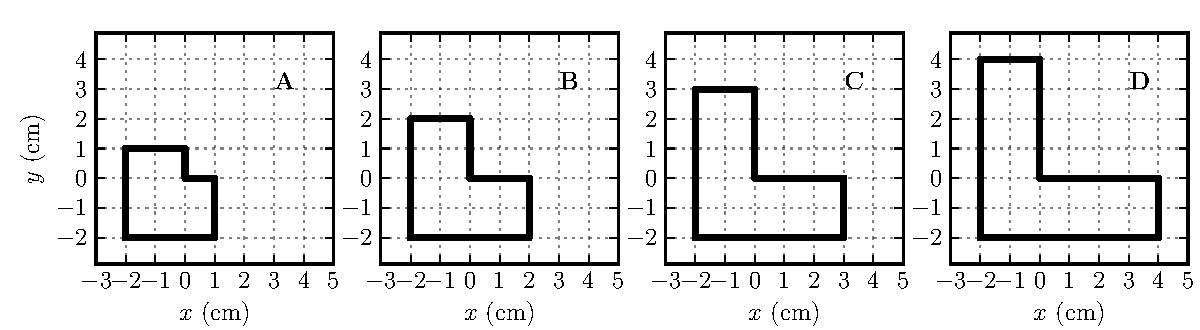
\includegraphics[width=\textwidth]{../py/com_shapes.pdf}\addtocounter{answer}{4}
  \answer{none of these}
  \end{answers}
\end{problem}

\begin{problem}
  \source{from problem set 7, problem 2} Just before jumping out of
  the way, a (daring) student throws a ball at $20\,\mi\,\h^{-1}$
  straight at a bus moving towards the student at $35\,\mi\,\h^{-1}$.
  Assume that these are the speeds just before the collision, that the
  collision is head-on, that the collision is elastic, and that the
  front of the bus is a flat, vertical plane.  Right after the
  collision (after the ball leaves contact with the bus), what will be
  the speed of the ball?  Give your answer for the original reference
  frame.
  \begin{answers}
    \answer{$60\,\mi\,\h^{-1}$}
    \answer{$70\,\mi\,\h^{-1}$}
    \answer{$80\,\mi\,\h^{-1}$}
    \answer{$90\,\mi\,\h^{-1}$}
    \answer{none of these}
  \end{answers}
\end{problem}

\begin{problem}
  \source{from problem set 8, problem 2} When you are holding a heavy
  grocery bag in your hand, and your arm is bent so that the upper arm
  is vertical and the forearm is horizontal, which of the following is
  true of the magnitude of the tension in your bicep and the magnitude
  of the weight of the bag?
  \begin{answers}
    \answer{the tension is much less than the weight}
    \answer{the tension is about the same as the weight}
    \answer{the tension is much more than the weight}
    \answer{it depends}
  \end{answers}
\end{problem}

\begin{problem}
  \source{from problem set 9, problem 2} A mass $m$ attached to a
  spring oscillates with amplitude $A$ (a length) and angular
  frequency $\omega$.  What is the total energy $E$ in the oscillator?
  \begin{answers}
    \answer{$\displaystyle E=\frac{1}{2}\,m\,\omega^2\,A^2$}
    \answer{$\displaystyle E=m\,\omega^2\,A^2$}
    \answer{$\displaystyle E=\frac{1}{2}\,k\,\omega^2\,A^2$}
    \answer{$\displaystyle E=k\,\omega^2\,A^2$}
    \answer{none of these}
  \end{answers}
\end{problem}

\begin{problem}
  \source{from problem set 10, problem 1} An organ pipe that plays
  middle $C$ is about 1.1 feet long.  How long would an organ pipe
  be that plays $C$ but one octave lower, that is, a factor of two
  lower in frequency?
  \begin{answers}
    \answer{0.55 feet}
    \answer{0.78 feet}
    \answer{1.1 feet}
    \answer{1.6 feet}
    \answer{2.2 feet}
  \end{answers}
\end{problem}

\begin{problem}
  \source{from problem set 11, problem 2} For a submerged ice cube in
  cold water, the gravitational force $|m\,\vec{g}|$ is smaller than the buoyant
  force $|\vec{F}_b|$.  What is the ratio $|m\,\vec{g}|/|\vec{F}_b|$?
  \begin{answers}
    \answer{0.92}
    \answer{0.42}
    \answer{0.08}
    \answer{0}
    \answer{nothing near any of these}
  \end{answers}
\end{problem}

\begin{problem}
  \source{from problem set 12, problem 2} If the kinematic viscosity
  $\nu$ is measured in units of $\m^2\,\s^{-1}$, then which of these
  formulae could represent a speed?  In these, $R$ is a length, and
  $g$ is an acceleration.
  \begin{answers}
    \answer{$\displaystyle\frac{g\,R^2}{\nu}$}
    \answer{$\displaystyle\frac{R}{\nu\,g}$}
    \answer{$\displaystyle\frac{g}{\nu\,R^2}$}
    \answer{$\displaystyle\frac{\nu}{g\,R}$}
    \answer{none of these}
  \end{answers}
\end{problem}

\end{document}
